\documentclass{article}

\usepackage{tikz} 
\usetikzlibrary{automata, positioning, arrows} 

\usepackage{amsthm}
\usepackage{amsfonts}
\usepackage{amsmath}
\usepackage{amssymb}
\usepackage{fullpage}
\usepackage{color}
\usepackage{parskip}
\usepackage{hyperref}

\usepackage{booktabs}

  \hypersetup{
    colorlinks = true,
    urlcolor = blue,       % color of external links using \href
    linkcolor= blue,       % color of internal links 
    citecolor= blue,       % color of links to bibliography
    filecolor= blue,       % color of file links
    }
    
\usepackage{listings}
\usepackage[utf8]{inputenc}                                                    
\usepackage[T1]{fontenc}                                                       

\definecolor{dkgreen}{rgb}{0,0.6,0}
\definecolor{gray}{rgb}{0.5,0.5,0.5}
\definecolor{mauve}{rgb}{0.58,0,0.82}

\lstset{frame=tb,
  language=haskell,
  aboveskip=3mm,
  belowskip=3mm,
  showstringspaces=false,
  columns=flexible,
  basicstyle={\small\ttfamily},
  numbers=none,
  numberstyle=\tiny\color{gray},
  keywordstyle=\color{blue},
  commentstyle=\color{dkgreen},
  stringstyle=\color{mauve},
  breaklines=true,
  breakatwhitespace=true,
  tabsize=3
}

\newtheoremstyle{theorem}
  {\topsep}   % ABOVESPACE
  {\topsep}   % BELOWSPACE
  {\itshape\/}  % BODYFONT
  {0pt}       % INDENT (empty value is the same as 0pt)
  {\bfseries} % HEADFONT
  {.}         % HEADPUNCT
  {5pt plus 1pt minus 1pt} % HEADSPACE
  {}          % CUSTOM-HEAD-SPEC
\theoremstyle{theorem} 
   \newtheorem{theorem}{Theorem}[section]
   \newtheorem{corollary}[theorem]{Corollary}
   \newtheorem{lemma}[theorem]{Lemma}
   \newtheorem{proposition}[theorem]{Proposition}
\theoremstyle{definition}
   \newtheorem{definition}[theorem]{Definition}
   \newtheorem{example}[theorem]{Example}
\theoremstyle{remark}    
  \newtheorem{remark}[theorem]{Remark}

\title{CPSC-354 Report}
\author{Nathan Garcia  \\ Chapman University}

\date{\today} 

\begin{document}

\maketitle

\begin{abstract}
\end{abstract}

\setcounter{tocdepth}{3}
\tableofcontents

\section{Introduction}\label{intro}

\section{Week by Week}\label{homework}

\subsection{Week 1}
\subsubsection{MU Puzzle}

The MU puzzle comes from the book \textit{Gödel, Escher, Bach}. You start with the string \textbf{MI} and the goal is to turn it into \textbf{MU} by following four rules:

\begin{enumerate}
    \item If a string ends with \textbf{I}, you can add a \textbf{U} at the end.  
    \item If a string starts with \textbf{M}, you can copy everything after the M.  
    \item If you see \textbf{III}, you can change it to \textbf{U}.  
    \item If you see \textbf{UU}, you can delete it.  
\end{enumerate}

The puzzle is about seeing if you can reach \textbf{MU} by only using these rules. It is not really about the letters themselves, but about how rules control what strings you can or cannot make.
\subsubsection{HW1}

The MU puzzle comes from the book \textit{Gödel, Escher, Bach}. You start with the string \textbf{MI} and the goal is to turn it into \textbf{MU} by following four rules:

\begin{enumerate}
    \item If a string ends with \textbf{I}, you can add a \textbf{U} at the end.  
    \item If a string starts with \textbf{M}, you can copy everything after the M.  
    \item If you see \textbf{III}, you can change it to \textbf{U}.  
    \item If you see \textbf{UU}, you can delete it.  
\end{enumerate}

At first, I tried small derivations. For example:
\[
\texttt{MI} \;\Rightarrow\; \texttt{MIU} \;\Rightarrow\; \texttt{MIUIU}
\]
or duplicating I’s:
\[
\texttt{MI} \;\Rightarrow\; \texttt{MII} \;\Rightarrow\; \texttt{MIIII}
\]
From \texttt{MIIII}, I can replace \texttt{III} with \texttt{U}, giving \texttt{MUI}, but not \texttt{MU}. Every time, an extra \texttt{I} is left over, and there is no rule that deletes a single \texttt{I}.

\paragraph{Invariant Argument.}  
Let $\#I(w)$ denote the number of \texttt{I}'s in string $w$. If we track $\#I(w) \pmod 3$, we find:
\begin{itemize}
    \item Rule 1: $\#I$ unchanged.  
    \item Rule 2: $\#I$ doubles. Over $\mathbb{Z}/3\mathbb{Z}$, $1 \mapsto 2$, $2 \mapsto 1$, never $0$.  
    \item Rule 3: Removes $3$ I’s, leaving the remainder mod 3 unchanged.  
    \item Rule 4: Deletes U’s only, so $\#I$ unchanged.  
\end{itemize}

We start with \texttt{MI}, which has $\#I=1$. This is congruent to $1 \pmod 3$. Because no rule ever makes $\#I \equiv 0 \pmod 3$, it is impossible to reach a string with $\#I=0$.

\paragraph{Conclusion.}  
The target \texttt{MU} has $\#I=0$, which is divisible by $3$. Since that is unreachable from \texttt{MI}, the puzzle is unsolvable. As a student, the cool part here is that the solution isn’t about brute-force trying rules—it’s about spotting a hidden invariant (the number of I’s mod 3) that blocks the path completely.

\subsection{Week 2}
\subsubsection{HW}

\paragraph{Problem.}
Consider the following list of Abstract Rewriting Systems (ARSs).
\begin{enumerate}
  \item $A=\varnothing$.
  \item $A=\{a\}$ \; and \; $R=\varnothing$.
  \item $A=\{a\}$ \; and \; $R=\{(a,a)\}$.
  \item $A=\{a,b,c\}$ \; and \; $R=\{(a,b),(a,c)\}$.
  \item $A=\{a,b\}$ \; and \; $R=\{(a,a),(a,b)\}$.
  \item $A=\{a,b,c\}$ \; and \; $R=\{(a,b),(b,b),(a,c)\}$.
  \item $A=\{a,b,c\}$ \; and \; $R=\{(a,b),(b,b),(a,c),(c,c)\}$.
\end{enumerate}

\noindent\textbf{Task.} Draw a picture for each ARS above (nodes = elements of $A$, arrows = pairs in $R$).
Then determine whether each ARS is \emph{terminating}, \emph{confluent}, and whether it has \emph{unique normal forms}.

% ---------- STYLE FOR ALL DIAGRAMS ----------
\tikzset{
  rsnode/.style = {circle, draw, minimum size=7mm, inner sep=0pt},
  rsgraph/.style = {->, thick, node distance=2.0cm}
}

\medskip

% ===== ARS 1 =====
\begin{center}
\begin{tikzpicture}[rsgraph]
  % A = empty set -> no nodes, just a label
  \node[draw=none] (lab) {\textbf{ARS 1:} $A=\varnothing$ (no elements to draw)};
\end{tikzpicture}
\end{center}

% ===== ARS 2 =====
\begin{center}
\begin{tikzpicture}[rsgraph]
  % A = {a}, R = empty (just one isolated node, no arrows)
  \node[rsnode] (a) {a};
  \node[draw=none, below=8pt of a] { \textbf{ARS 2:} $A=\{a\},\ R=\varnothing$ };
\end{tikzpicture}
\end{center}

% ===== ARS 3 =====
\begin{center}
\begin{tikzpicture}[rsgraph]
  % A = {a}, R = {(a,a)}  -- single node with a self-loop
  \node[rsnode] (a) {a};
  \path (a) edge[loop right] (a);
\end{tikzpicture}

\smallskip
\textbf{ARS 3:} $A=\{a\},\ R=\{(a,a)\}$
\end{center}


% ===== ARS 4 =====
\begin{center}
\begin{tikzpicture}[rsgraph]
  % A = {a,b,c}, R = {(a,b),(a,c)}
  \node[rsnode] (a) {a};
  \node[rsnode, below left=1.2cm and 1.2cm of a] (b) {b};
  \node[rsnode, below right=1.2cm and 1.2cm of a] (c) {c};
  \path (a) edge (b)
        (a) edge (c);
  \node[draw=none, below=8pt of b.center, xshift=1.2cm] { \textbf{ARS 4:} $A=\{a,b,c\},\ R=\{(a,b),(a,c)\}$ };
\end{tikzpicture}
\end{center}

% ===== ARS 5 =====
\begin{center}
\begin{tikzpicture}[rsgraph]
  % A = {a,b}, R = {(a,a),(a,b)}
  \node[rsnode] (a) {a};
  \node[rsnode, right=2.5cm of a] (b) {b};
  \path (a) edge[loop above] (a)
        (a) edge (b);
  \node[draw=none, below=8pt of a, xshift=1.25cm] { \textbf{ARS 5:} $A=\{a,b\},\ R=\{(a,a),(a,b)\}$ };
\end{tikzpicture}
\end{center}

% ===== ARS 6 =====
\begin{center}
\begin{tikzpicture}[rsgraph]
  % A = {a,b,c}, R = {(a,b),(b,b),(a,c)}
  \node[rsnode] (a) {a};
  \node[rsnode, below left=1.2cm and 1.2cm of a] (b) {b};
  \node[rsnode, below right=1.2cm and 1.2cm of a] (c) {c};
  \path (a) edge (b)
        (a) edge (c)
        (b) edge[loop left] (b);
  \node[draw=none, below=8pt of b.center, xshift=1.2cm] { \textbf{ARS 6:} $A=\{a,b,c\},\ R=\{(a,b),(b,b),(a,c)\}$ };
\end{tikzpicture}
\end{center}

% ===== ARS 7 =====
\begin{center}
\begin{tikzpicture}[rsgraph]
  % A = {a,b,c}, R = {(a,b),(b,b),(a,c),(c,c)}
  \node[rsnode] (a) {a};
  \node[rsnode, below left=1.2cm and 1.2cm of a] (b) {b};
  \node[rsnode, below right=1.2cm and 1.2cm of a] (c) {c};
  \path (a) edge (b)
        (a) edge (c)
        (b) edge[loop left] (b)
        (c) edge[loop right] (c);
  \node[draw=none, below=8pt of b.center, xshift=1.2cm] { \textbf{ARS 7:} $A=\{a,b,c\},\ R=\{(a,b),(b,b),(a,c),(c,c)\}$ };
\end{tikzpicture}
\end{center}


\begin{center}
\begin{tabular}{@{}lccc@{}}
\toprule
\textbf{ARS} & \textbf{Terminating} & \textbf{Confluent} & \textbf{Has Unique Normal Forms} \\
\midrule
1 & \phantom{True/False}X & \phantom{True/False}X & \phantom{True/False}X \\
2 & X & X & X \\
3 &  & X &  \\
4 & X &  & X \\
5 &  & X & X \\
6 &  &  &  \\
7 &  &  &  \\
\bottomrule
\end{tabular}
\end{center}
\begin{enumerate}
  \item \textbf{Confluent: True}, \textbf{Terminating: True}, \textbf{Unique Normal Forms: False}\\
  % This is not possible
  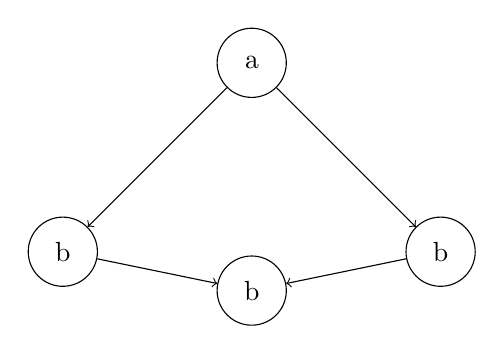
\begin{tikzpicture}[->, node distance=2.5cm]
    \node[state] (a) {a};
    \node[state, below left=of a] (b1) {b};
    \node[state, below right=of a] (b2) {b};
    \node[state, below=2cm of a] (b3) {b};
    \draw (a) -- (b1);
    \draw (a) -- (b2);
    \draw (b1) -- (b3);
    \draw (b2) -- (b3);
  \end{tikzpicture}

  \item \textbf{Confluent: True}, \textbf{Terminating: False}, \textbf{Unique Normal Forms: True}\\
  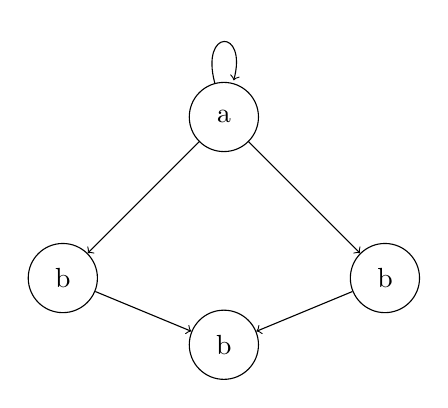
\begin{tikzpicture}[->, node distance=2cm]
    \node[state] (a) {a};
    \node[state, below left=of a] (b1) {b};
    \node[state, below right=of a] (b2) {b};
    \node[state, below=2cm of a] (b3) {b};
    \draw (a) -- (b1);
    \draw (a) -- (b2);
    \draw (b1) -- (b3);
    \draw (b2) -- (b3);
    \draw (a) edge[loop above] (a);
  \end{tikzpicture}

  \item \textbf{Confluent: True}, \textbf{Terminating: False}, \textbf{Unique Normal Forms: False}\\
  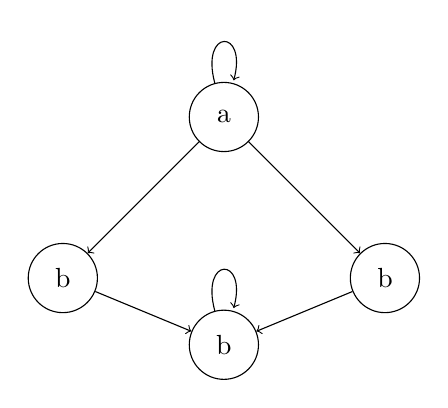
\begin{tikzpicture}[->, node distance=2cm]
    \node[state] (a) {a};
    \node[state, below left=of a] (b1) {b};
    \node[state, below right=of a] (b2) {b};
    \node[state, below=2cm of a] (b3) {b};
    \draw (a) -- (b1);
    \draw (a) -- (b2);
    \draw (b1) -- (b3);
    \draw (b2) -- (b3);
    \draw (a) edge[loop above] (a);
    \draw (b3) edge[loop above] (b3);
  \end{tikzpicture}

  \item \textbf{Confluent: False}, \textbf{Terminating: True}, \textbf{Unique Normal Forms: True}\\
  \begin{tikzpicture}[->, node distance=2cm]
    \node[state] (a) {a};
    \node[state, below right=of a] (b) {b};
    \draw (a) -- (b);
  \end{tikzpicture}

  \item \textbf{Confluent: False}, \textbf{Terminating: True}, \textbf{Unique Normal Forms: False}\\
  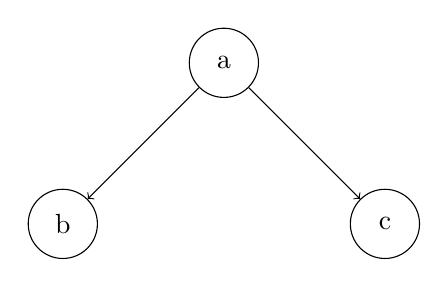
\begin{tikzpicture}[->, node distance=2cm]
    \node[state] (a) {a};
    \node[state, below left=of a] (b) {b};
    \node[state, below right=of a] (c) {c};
    \draw (a) -- (b);
    \draw (a) -- (c);
  \end{tikzpicture}

  \item \textbf{Confluent: False}, \textbf{Terminating: False}, \textbf{Unique Normal Forms: True}\\
  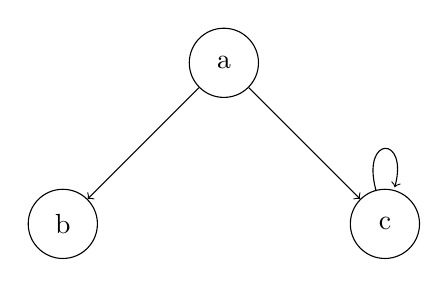
\begin{tikzpicture}[->, node distance=2cm]
    \node[state] (a) {a};
    \node[state, below left=of a] (b) {b};
    \node[state, below right=of a] (c) {c};
    \draw (a) -- (b);
    \draw (a) -- (c);
    \draw (c) edge[loop above] (c);
  \end{tikzpicture}

  \item \textbf{Confluent: False}, \textbf{Terminating: False}, \textbf{Unique Normal Forms: False}\\
  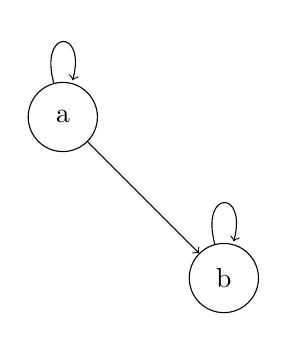
\begin{tikzpicture}[->, node distance=2cm]
    \node[state] (a) {a};
    \node[state, below right=of a] (b) {b};
    \draw (a) -- (b);
    \draw (a) edge[loop above] (a);
    \draw (b) edge[loop above] (b);
  \end{tikzpicture}
\end{enumerate}

\subsection{HW 3}
\subsubsection{Exercise 5}
\textbf{Exercise 5.}

\textit{Rules:}
\[
ab \to ba, \quad ba \to ab, \quad aa \to \epsilon, \quad b \to \epsilon
\]

\textit{Sample reductions:}
\[
abba \;\to\; bbaa \;\to\; baa \;\to\; aa \;\to\; \epsilon
\]
\[
bababa \;\to\; aaabbb \;\to\; aabbb \;\to\; abbb \;\to\; a
\]

\textit{Non-termination:} The rules $ab \to ba$ and $ba \to ab$ form an infinite loop:
\[
ab \to ba \to ab \to ba \to \cdots
\]

\textit{Non-equivalent strings:} $a$ and $\epsilon$ are not equivalent, since a single $a$ cannot be eliminated.

\textit{Equivalence classes:}  
Order does not matter (due to swapping).  
$b$’s vanish.  
$aa \to \epsilon$ ensures only the \emph{parity} of the number of $a$’s matters.  

\[
I(w) = \#a(w) \bmod 2 \in \{0,1\}
\]

Thus there are exactly two equivalence classes:
\[
\{w \mid \#a(w) \equiv 0 \pmod 2\} \quad\longmapsto\quad \epsilon
\]
\[
\{w \mid \#a(w) \equiv 1 \pmod 2\} \quad\longmapsto\quad a
\]

\textit{Modified terminating system:}
\[
ab \to ba, \quad aa \to \epsilon, \quad b \to \epsilon
\]
Termination follows from length and inversion-count measures.  

\textit{Specification:} The algorithm computes the \emph{parity of the number of $a$’s}, ignoring $b$’s.

\vspace{1em}

\textbf{Exercise 5b.}

\textit{Rules:}
\[
ab \to ba, \quad ba \to ab, \quad aa \to a, \quad b \to \epsilon
\]

\textit{Sample reductions:}
\[
abba \;\to\; bbaa \;\to\; baa \;\to\; aa \;\to\; a
\]
\[
bababa \;\to\; aaabbb \;\to\; aabbb \;\to\; abbb \;\to\; a
\]

\textit{Non-termination:} As before, infinite swapping is possible.

\textit{Non-equivalent strings:} $\epsilon$ and $a$ are not equivalent: all $b$’s vanish, and any positive number of $a$’s reduces to $a$.

\textit{Equivalence classes:}  
Order does not matter.  
$b$’s vanish.  
$aa \to a$ collapses any positive number of $a$’s to a single $a$.  

\[
J(w) =
\begin{cases}
0 & \text{if } \#a(w) = 0 \\
1 & \text{if } \#a(w) \geq 1
\end{cases}
\]

Thus there are exactly two equivalence classes:
\[
\{w \mid \#a(w) = 0\} \quad\longmapsto\quad \epsilon
\]
\[
\{w \mid \#a(w) \geq 1\} \quad\longmapsto\quad a
\]

\textit{Modified terminating system:}
\[
ab \to ba, \quad aa \to a, \quad b \to \epsilon
\]
This terminates and yields unique normal forms.  

\textit{Specification:} The algorithm computes whether the input contains at least one $a$, ignoring all $b$’s.

\subsection{Week 4}
\subsubsection{hw4}
\subsubsection*{HW 4, PL 2025, Termination}
For the definition of a \emph{measure function}, see our notes on rewriting and, in particular, on termination.

\paragraph{HW 4.1.}
Consider the following algorithm (Euclid’s algorithm for the greatest common divisor):

\begin{verbatim}
while b != 0:
    temp = b
    b = a mod b
    a = temp
return a
\end{verbatim}

\textbf{Conditions.} Assume inputs $a,b \in \mathbb{N}$ with $b \geq 0$ and the usual remainder operation, i.e.\ for $b>0$ we have $0 \leq a \bmod b < b$. (If $b=0$, the loop is skipped and the algorithm terminates immediately.)

\textbf{Measure function.} Define
\[
\mu(a,b) := b \in \mathbb{N}.
\]

\textbf{Proof of termination.}  
If the loop guard holds ($b \neq 0$), one iteration maps the state $(a,b)$ to
\[
(a',b') = (\,b,\ a \bmod b\,).
\]
By the property of the remainder,
\[
0 \leq b' = a \bmod b < b = \mu(a,b).
\]
Thus $\mu$ strictly decreases on every loop iteration and is bounded below by $0$.  
Since $(\mathbb{N},<)$ is well-founded, no infinite descending chain
\[
\mu(a_0,b_0) > \mu(a_1,b_1) > \mu(a_2,b_2) > \cdots
\]
exists. Hence only finitely many iterations are possible; the loop terminates and the algorithm halts. \qed

\medskip

\paragraph{HW 4.2.}
Consider the following fragment of merge sort:

\begin{verbatim}
function merge_sort(arr, left, right):
    if left >= right:
        return
    mid = (left + right) / 2
    merge_sort(arr, left, mid)
    merge_sort(arr, mid+1, right)
    merge(arr, left, mid, right)
\end{verbatim}

Define
\[
\phi(left,right) := right - left + 1.
\]

\textbf{Claim.} $\phi$ is a measure function for \texttt{merge\_sort}.

\textbf{Proof.}
\begin{itemize}
    \item \emph{Well-defined, nonnegative.} For valid indices with $left \leq right$, we have $\phi(left,right) \in \mathbb{N}$ and $\phi \geq 1$. If $left > right$ the function is not called (or $\phi \leq 0$, and the base case applies immediately).
    \item \emph{Base case.} When $left \geq right$, the function returns immediately; in this case $\phi(left,right) \leq 1$, i.e.\ there is no further recursion.
    \item \emph{Strict decrease on recursive calls.} Suppose $left < right$ and let $n := \phi(left,right) = right-left+1 \geq 2$. With $mid = \lfloor (left+right)/2 \rfloor$:
    \[
    \phi(left,mid) = mid - left + 1 \leq \left\lfloor \tfrac{n}{2} \right\rfloor < n,
    \]
    \[
    \phi(mid+1,right) = right - (mid+1) + 1 = right - mid \leq \left\lceil \tfrac{n}{2} \right\rceil < n.
    \]
    Thus both recursive calls strictly reduce the measure.
\end{itemize}

Since $\phi$ maps each call to a natural number that strictly decreases along every recursive edge and is bounded below, there are no infinite descending chains. By well-founded induction on $\phi$, all recursive calls terminate. \qed

\subsection{HW 5}
\subsubsection*{Workout: Step-by-step $\alpha$/$\beta$-reductions}

\noindent\textbf{Problem.} Evaluate
\[
(\lambda f.\,\lambda x.\,f(f\,x))\;(\lambda f.\,\lambda x.\,f(f(f\,x))).
\]

\noindent\textbf{Notation.}
We use $\rightsquigarrow_\beta$ for a single $\beta$-reduction step and “$\alpha$” to indicate a capture-avoiding renaming of bound variables.

\noindent\textbf{Intuition.}
The term $\lambda f.\,\lambda x.\,f(f\,x)$ applies a function twice (\emph{iterate-2}).  
The term $\lambda f.\,\lambda x.\,f(f(f\,x))$ applies a function three times (\emph{iterate-3}).  
Applying iterate-2 \emph{to} iterate-3 yields iterate-9.

\noindent\textbf{Derivation.}
\begin{align*}
&(\lambda f.\,\lambda x.\,f(f\,x))\;(\lambda f.\,\lambda x.\,f(f(f\,x)))\\[2pt]
&\rightsquigarrow_\beta\ \lambda x.\, \big[(\lambda f.\,\lambda x.\,f(f(f\,x)))\big((\lambda f.\,\lambda x.\,f(f(f\,x)))\,x\big)\big]
\quad\text{(substitute $f := \lambda f.\lambda x.\,f(f(f\,x))$ into $\lambda x.\,f(f\,x)$)}\\[4pt]
&\overset{\alpha}{=}\ \lambda x.\, (\lambda f.\,\lambda y.\,f(f(f\,y)))\Big((\lambda f.\,\lambda u.\,f(f(f\,u)))\,x\Big)
\quad\text{(rename bound $x$'s to $y,u$ to avoid shadowing)}\\[4pt]
&\rightsquigarrow_\beta\ \lambda x.\, (\lambda f.\,\lambda y.\,f(f(f\,y)))\big(\lambda u.\,x(x(x\,u))\big)
\quad\text{(apply $\beta$ to $(\lambda f.\lambda u.\,f(f(f\,u)))\,x$)}\\[4pt]
&\rightsquigarrow_\beta\ \lambda x.\,\lambda y.\,F\big(F(F\,y)\big)
\quad\text{with }F:=\lambda u.\,x(x(x\,u))
\quad\text{(apply $(\lambda f.\lambda y.\,f(f(f\,y)))\,F$)}\\[4pt]
&=\ \lambda x.\,\lambda y.\,F\Big(F\big(F\,y\big)\Big)\\[2pt]
&=\ \lambda x.\,\lambda y.\,F\Big(F\big(x(x(x\,y))\big)\Big)
\quad\text{(since $F\,y = x(x(x\,y))$)}\\[2pt]
&=\ \lambda x.\,\lambda y.\,F\Big(x\big(x\big(x\big(x(x(x\,y))\big)\big)\big)\Big)
\quad\text{(apply $F$ again; adds $3$ more $x$'s: total $6$)}\\[2pt]
&=\ \lambda x.\,\lambda y.\,x\big(x\big(x\big(x\big(x\big(x\big(x\big(x\big(x\,y\big)\big)\big)\big)\big)\big)\big)\big)
\quad\text{(apply $F$ a third time; +3 more: total $9$)}.
\end{align*}

\noindent\textbf{Normal form.}
\[
\boxed{\ \lambda x.\,\lambda y.\,\underbrace{x(x(x(x(x(x(x(x(x\,y))))))))}_{\text{$9$ applications of }x}\ }
\]
So the result is the \emph{iterate-9} operator: given $x$ and $y$, it applies $x$ to $y$ nine times.


\section{Essay}

\section{Evidence of Participation}

\section{Conclusion}\label{conclusion}

\begin{thebibliography}{99}
\bibitem[BLA]{bla} Author, \href{https://en.wikipedia.org/wiki/LaTeX}{Title}, Publisher, Year.
\end{thebibliography}

\end{document}
